
\documentclass[14pt, a2paper, portrait]{tikzposter}

\usepackage[brazil]{babel}
\usepackage[utf8]{inputenc}
\usepackage[T1]{fontenc}
\usepackage{lipsum}
 
\newcommand{\bs}{\textbackslash}   
\newcommand{\cmd}[1]{{\bf \color{red}#1}}   
\tikzposterlatexaffectionproofon

\title{Projeto Integrador 3° Sem. - Cartagena }

\author{Guilherme Silva, Gustavo Pardini, Henrique Marques, Théo Bortoletto} 

\institute{Centro Universitário Senac}

 % Set colortheme
 % (default, anil, armin, edgar, emre, hanna, james, kai, lena, manuel,
 % martin, max, nicolas, pascal, peter, philipp, richard, roman, stefanie,
 % vinay)
\usecolortheme{edgar}

\definecolor{framecolor}{named}{black}



\begin{document}

\titleblock[left fig=logo.PNG, embedded]

\block[l]{Introdução}{
   Neste semestre (3°), tivemos que fazer um sistema autônomo que jogaria um jogo de tabuleiro. E o jogo de escolhido foi o "Cartagena". O objetivo do jogo é ajudar seus piratas a escapar da prisão na caverna e ser o primeiro a conseguir que todos eles cheguem ao barco no final do caminho
   \newline
   Durante o jogo, os jogadores jogam cartas para mover seus piratas ao longo do caminho. Cada carta tem um símbolo que corresponde a uma cor do caminho, permitindo que o jogador mova um pirata para a próxima casa nessa cor. O objetivo é mover seus piratas habilmente, usando as cartas disponíveis, para alcançar a saída.
}

\begin{columns}
% 1a coluna
\column{0.48}

\block[c]{Estratégia Implementada}{

  A estratégia que implementamos consiste em: 
  \begin{tipo da lista}
   \item - verificar se há a possibilidade de voltar para ganhar duas cartas. Caso tenha, o pirata volta e ganha duas cartas.
   \item - caso não tenha a possibilidade de ganhar duas cartas, o sistema tenta jogar o pirata da última casa por uma sequência definida de cartas (na ordem Esqueleto, Faca, Garrafa, Chave, Tricórnio e Pistola).
   \item - caso não haja cartas, o pirata que está mais longe volta para ganhar uma carta.
 \end{tipo da lista}

}
% 2a coluna
\column{0.52}

\block[c]{Resultado}{
   Este é o resultado do sistema sendo compilado dentro de uma partida. É possível observar o tabuleiro, as cartas, a quantidade de cartas, a quantidade de piratas na partida.
   \newline
   
        \centering
        \includegraphics[scale = 0.3]{ingame.png}

}
\end{columns}

\column{0.5}
\block [c, width=30cm] {Considerações Finais}{
   Foi usado como linguagem principal o "C#" para a realização deste projeto, fazendo o uso de "orientação de objetos" vistos em sala de aula durante todo o semestre. Também foi o utilizado o Figma, uma ferramenta de design, para fazer a parte visual do projeto.
}


\block[c,width=30cm]{Referências}{

\begin{center}

\includegraphics[scale=0.2]{c#.png}
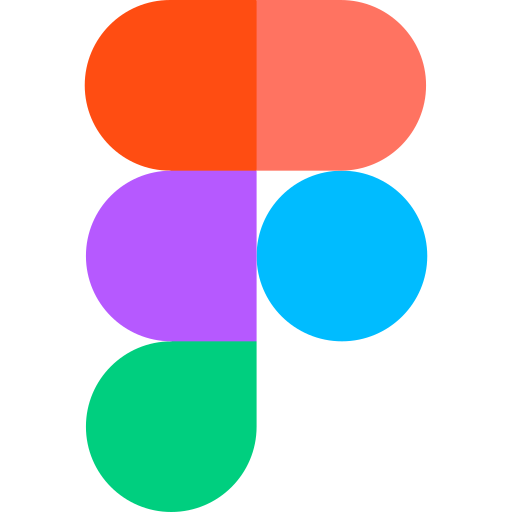
\includegraphics[scale=0.2]{figma.png}

\includegraphics[scale=0.1]{visualstudio.png}

\end{center}

}

\end{document}


